\documentclass[10pt,twocolumn]{article} 

% use the oxycomps style file
\usepackage{oxycomps}

% import packages for listing code
\usepackage{listings}
\usepackage{xcolor}
\usepackage{color}
\usepackage{listings}    
\usepackage{courier}

% define colors for code segments
\definecolor{codegreen}{rgb}{0,0.6,0}
\definecolor{codegray}{rgb}{0.5,0.5,0.5}
\definecolor{codepurple}{rgb}{0.58,0,0.82}
\definecolor{backcolour}{rgb}{0.95,0.95,0.92}
\definecolor{arduinoGreen}{rgb}{0.17,0.43,0.01}
\definecolor{arduinoGrey}{rgb}{0.47,0.47,0.33}
\definecolor{arduinoOrange}{rgb}{0.8,0.4,0}
\definecolor{arduinoBlue}{rgb}{0.01,0.61,0.98}
\definecolor{arduinoDarkBlue}{rgb}{0.0,0.2,0.5}

% define code style
\lstdefinestyle{python}{
    backgroundcolor=\color{backcolour},   
    commentstyle=\color{codegreen},
    keywordstyle=\color{magenta},
    numberstyle=\tiny\color{codegray},
    stringstyle=\color{codepurple},
    basicstyle=\ttfamily\footnotesize,
    breakatwhitespace=false,         
    breaklines=true,                 
    captionpos=b,                    
    keepspaces=true,                 
    numbers=left,                    
    numbersep=5pt,                  
    showspaces=false,                
    showstringspaces=false,
    showtabs=false,                  
    tabsize=2
}

% use hyperref package
\usepackage{hyperref}

% read references.bib for the bibtex data
\bibliography{references}

% include metadata in the generated pdf file
\pdfinfo{
    /Title (The Occidental Computer Science Comprehensive Project: Tutorial)
    /Author (Odelia Putterman)
}

% set the title and author information
\title{The Occidental Computer Science Comprehensive Project: \\ Tutorial Report}
\author{Odelia Putterman}
\affiliation{Occidental College}
\email{putterman@oxy.edu}

\begin{document}

\maketitle

\begin{abstract}
    This report documents the tutorial completed as part of my Occidental College Computer Science Comprehensive Project: \textit{Predicting Cryptocurrency Prices for Stock Trading Using Machine Learning}. This report has four components: methods, evaluation, discussion, and software documentation. For each component, we include a section. This report walks us through the tutorial followed, \href{https://www.youtube.com/watch?v=4OlvGGAsj8I}{Stock Market Sentiment Analysis Using Python \& Machine Learning (Youtube tutorial)}, reviewing the key concepts and learned information relevant to the comprehensive project.
\end{abstract}

\section{Methods}

This section is a walk-through of the methods implored in this tutorial in a numbered list. This tutorial was done in Google Colab. We detail the steps below.

\begin{enumerate}
    \item First, we installed \textit{vaderSentiment} with pip to get access to sentiment analysis tools. These will be used later on in the tutorial.
    
\lstset{style=python}

\begin{lstlisting}[language=Python, caption=Install vaderSentiment]
pip install vaderSentiment
\end{lstlisting}

    \item Next, we load all the necessary libraries for this tutorial. These are:
    \begin{itemize}
        \item pandas;
        \item numpy;
        \item textblob.TextBlob;
        \item re;
        \item vaderSentiment.SentimentIntensityAnalyzer;
        \item sklearn.model\_selection.train\_test\_split;
        \item sklearn.metrics.accuracy\_score;
        \item sklearn.metrics.classification\_report; and
        \item sklearn.discriminant\_analysis.LinearDiscriminantAnalysis.
    \end{itemize}

\begin{lstlisting}[language=Python, caption=Load Libraries]
#Import the libraries
import pandas as pd
import numpy as np
from textblob import TextBlob
import re
from vaderSentiment.vaderSentiment import SentimentIntensityAnalyzer
from sklearn.model_selection import train_test_split
from sklearn.metrics import accuracy_score, classification_report
from sklearn.discriminant_analysis import LinearDiscriminantAnalysis
\end{lstlisting}

    \item Next, we load in all the data for this tutorial using \textbf{google.colab.files.upload()}. There were two input data sets, which are the \textit{Dow\_Jones\_Industrial\_Average\_News.csv} and the \textit{Dow\_Jones\_Industrial\_Average\_Stock.csv}, all originating from data from the Dow Jones and downloaded from Kaggle at this link: \url{https://www.kaggle.com/datasets/aaron7sun/stocknews}.

\begin{lstlisting}[language=Python, caption=Upload data sets]
#Load the data
from google.colab import files
files.upload()
\end{lstlisting}

    \item Next, we merged these two data sets into a pandas data frame called \textit{merge} on the 'Date' field to consolidate our data. Now, this \textit{merge} data frame had the original news headers, label, date, open, high, low, close, volume, and adjacent close columns.

\begin{lstlisting}[language=Python, caption=Store and merge data]
#Store the data into variables
df1 = pd.read_csv('Dow_Jones_Industrial_Average_News.csv')
df2 = pd.read_csv('Dow_Jones_Industrial_Average_Stock.csv')

#Merge the data set on the date field
merge = df1.merge(df2, how='inner', on='Date')
\end{lstlisting}

    \item To prepare the data for sentiment analysis, we grabbed the \textit{news} data set inputs, consolidated them into one joint string for each date, and cleaned the data by removing certain unnecessary string patterns, storing this processed data in a new list and adding it to our consolidated csv under a new column called 'Combined\_News'. Now, the merged data frame had the original news headers, label, date, open, high, low, close, volume, and adjacent close columns in addition to newly added 'Combined\_News' column.

\begin{lstlisting}[language=Python, caption=Pre-process data]
#Combine the top news headlines
headlines = []

for row in range(0, len(merge.index)):
  headlines.append(' '.join( str(x) for x in merge.iloc[row, 2:27]))
 
#Clean the data
clean_headlines = []

for i in range(0, len(headlines)):
  clean_headlines.append(re.sub("b[(')]", '', headlines[i])) # remove b'
  clean_headlines[i] = re.sub('b[(")]', '', clean_headlines[i]) # remove b"
  clean_headlines[i] = re.sub("\'", '', clean_headlines[i]) #remove \'

#Add the clean headlines to the merge data set
merge['Combined_News'] = clean_headlines
\end{lstlisting}

    \item Next, we created functions to get the subjectivity and polarity of text using \textbf{TextBlob(text).sentiment.subjectivity} and \textbf{TextBlob(text).sentiment.polarity}, where \textbf{text} is replaced with the actual text to analyze.

\begin{lstlisting}[language=Python, caption=Subjectivity and polarity functions]
#Create a function to get the subjectivity
def getSubjectivity(text):
  return TextBlob(text).sentiment.subjectivity

#Create a function to get the polarity
def getPolarity(text):
  return TextBlob(text).sentiment.polarity
\end{lstlisting}

    \item We used these newly created functions to create a subjectivity and polarity column, called 'Subjectivity' and 'Polarity' respectively, with inputs as the subjectivity and polarity outputs from these functions on each line of 'Combined\_News' (the cleaned news string).

\begin{lstlisting}[language=Python, caption=Get subjectivity and polarity]
#Create two new columns 'Subjectivity' and 'Polarity'
merge['Subjectivity'] = merge['Combined_News'].apply(getSubjectivity)
merge['Polarity'] = merge['Combined_News'].apply(getPolarity)
\end{lstlisting}

    \item Next, we made a function to get the sentiment scores called \textbf{getSIA}. Using this function, we got the sentiment scores for each date, creating a new column in the combined csv for each of: 'combined', 'negative', 'neutral', and 'positive', where each is a value between -1 and 1.

\begin{lstlisting}[language=Python, caption=Add sentiment scores]
#Create a function to get the sentiment scores
def getSIA(text):
  sia = SentimentIntensityAnalyzer()
  sentiment = sia.polarity_scores(text)
  return sentiment
  
#Get the sentiment scores for each day
compound = []
neg = []
pos = []
neu = []
SIA = 0

for i in range(0, len(merge['Combined_News'])):
  SIA = getSIA(merge['Combined_News'][i])
  compound.append(SIA['compound'])
  neg.append(SIA['neg'])
  neu.append(SIA['neu'])
  pos.append(SIA['pos'])

#Store the sentiment scores in the merge data set
merge['Compound'] = compound
merge['Negative'] = neg
merge['Neutral'] = neu
merge['Positive'] = pos
\end{lstlisting}

    \item We cleaned our combined csv to keep only the necessary columns: 'Open', 'High', 'Low', 'Volume', 'Subjectivity', 'Polarity', 'Compound', 'Negative', 'Neutral', 'Positive', and 'Label'.

\begin{lstlisting}[language=Python, caption=Keep only necessary columns]
#Create a list of columns to keep
keep_columns = ['Open', 'High', 'Low', 'Volume', 'Subjectivity', 'Polarity', 'Compound', 'Negative', 'Neutral', 'Positive', 'Label']

df = merge[keep_columns]
\end{lstlisting}

    \item We split this cleaned combined csv into two data frames, one for the 'input' data (everything but the 'Label' column) and one for the target data (the 'Label' columns).

\begin{lstlisting}[language=Python, caption=Split into input and target data]
#Create the feature data set
X = df
X = np.array(X.drop(['Label'], 1))

#Create the target data set
y = np.array(df['Label'])
\end{lstlisting}

    \item Using \textbf{train\_test\_split}, we split the data into 80 percent and 20 percent to train and test the data.

\begin{lstlisting}[language=Python, caption=Split data into training and test]
#Split the data into 80% training and 20% testing data sets
x_train, x_test, y_train, y_test = train_test_split(X, y, test_size = 0.2, random_state = 0)
\end{lstlisting}

    \item Using the train data, we trained a \textbf{LinearDiscriminantAnalysis()} model.

\begin{lstlisting}[language=Python, caption=Train model]
#Create and train the model
model = LinearDiscriminantAnalysis().fit(x_train, y_train)
\end{lstlisting}

    \item And, finally, we got the model predictions for the test data and compared between these predictions and the labeled data to get the precision, recall, f1-score, and support.

\begin{lstlisting}[language=Python, caption=Get predictions and evaluate]
#Show the models predictions
predictions = model.predict(x_test)

#Show the model metrics
print(classification_report(y_test, predictions))
\end{lstlisting}

\end{enumerate}


\section{Evaluation}

This tutorial evaluated its outputted results by comparing the predicted stock prices produced from the trained model with the actual stock prices from that same period. This found to produce a precision rate over 80\%. Other measures besides precision were accounted for as well, including recall, f1-score, and support, all showing very promising results.

To evaluate our results, we split the data into 80\% training data and 20\% testing data using \textbf{train\_test\_split} from \textbf{sklearn.model\_selection}. After training the model using \textbf{LinearDiscriminantAnalysis()} on the training data, we used the model to make predictions for this test data. Next, we pulled the actual price changes from this time (on the 0/1 scale) and used \textbf{classification\_report} from \textbf{sklearn.metrics} to get the precision, recall, f1-score, support, accuracy, macro average, and weighted average, which are all metrics we can use to evaluate the success of our model which were, as mentioned, highly promising.

\begin{figure}
    \centering
    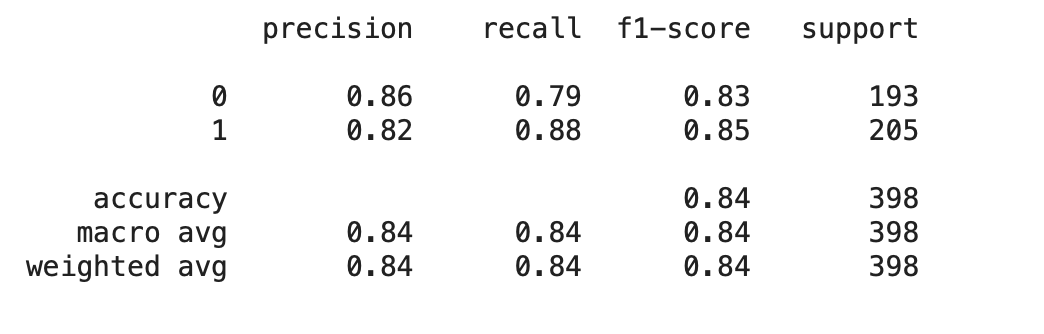
\includegraphics[scale=0.50]{images/evaluation_results.png}
    \caption{
        Evaluation metrics for tutorial results.
    }
\end{figure}

\section{Discussion}

Considering the relatively small size of the initial inputted data sets (less than 5.5 MB combined), I am very impressed with the high accuracy rates. Moreover, the tutorial was only trained on 80\% of this input data, meaning even less data was used in getting these impressive results. One the one hand, this tutorial leads me to believe that with the right input data, you do not need an enormous data set, but on the other hand, it suggests that if we collect even more relevant data, we can get even more outstanding results.

All that said, I have a few critiques for this tutorial's input formatting and outputted results. The result outputs simply gave a '0' or '1', where zero signified decreasing stock price and one stood for increasing stock price. This zero or one system is not very insightful, as we do not know \textit{how much} the stock is increasing or decreasing in price. If we could replace this system with a percentage of growth or decay, we could get more insightful data for the accuracy rates of our model but also for what to do with the results. As such, I would opt to switch the input stock price growth column with a numeric percentage in place of its current zero or one ranking. In doing so, our outputs would vary dramatically in projected percentage increase or decrease, allowing us to make more educated decisions and better evaluate the model's true accuracy.

Another critique I have is for the input data processing. In pre-processing the inputted file \textit{Dow\_Jones\_Industrial\_Average\_News.csv}, we processed the file to remove unnecessary, often repeated characters. Though this worked in this context because we knew the exact format of the input data, I would suggest using a preset list of words or character symbols to filter out on instead so we can account for unforeseen but potentially problematic tokens.

This tutorial walked me through how to predict stock prices (whether they will increase or decrease) with sentiment analysis based on top news headlines. The whole process was so seamless and straight-forward it boosted my confidence in my ability to carry-out this project tremendously. While it showed the ease with which sentiment analysis and model building can be done using pre-built libraries, it did not cover the complexity involved with sourcing data, as these data sets were simply provided in a form which was easy to work with. That said, data processing was covered, which is essential to the success of the model.

\section{Software Documentation}

See attached \textbf{stock\_market\_tutorial.pdf} file for the code from this tutorial.


\printbibliography 

\end{document}